\appendix

\chapter{Hojas de datos}
\label{chap:anexo-datasheets}

Las hojas de datos de los componentes activos principales empleados en las distintas etapas se encuentran disponibles
en la bibliografía técnica del proyecto:
\begin{itemize}
  \item LM324 / LM324N: Cuádruple amplificador operacional de alimentación simple ($\SI{3}{\volt}$ a
    $\SI{32}{\volt}$), entrada con rango de modo común hasta masa ($\SI{0}{\volt}$), empleado en la etapa de
    acondicionamiento de señal de campo de $\SI{4}{\milli\ampere}$ a $\SI{20}{\milli\ampere}$.
  \item TL084 / TL084CN: Cuádruple amplificador operacional con entradas JFET de ultra alta impedancia
    ($\approx \SI{1}{\tera\ohm}$), baja distorsión armónica, producto ganancia-ancho de banda
    $\text{GBW} = \SI{3}{\mega\hertz}$ y velocidad de respuesta $\text{SR} = \SI{13}{\volt/\micro\second}$, empleado
    en los filtros activos de 4.\textsuperscript{to} orden.
  \item BC337: Transistor bipolar NPN para la etapa 3 sumidero de corriente en el lazo industrial.
\end{itemize}

\chapter{Placa del filtro de señal de campo}
\label{chap:anexo-pcb-campo}

\begin{figure}[H]
  \centering
  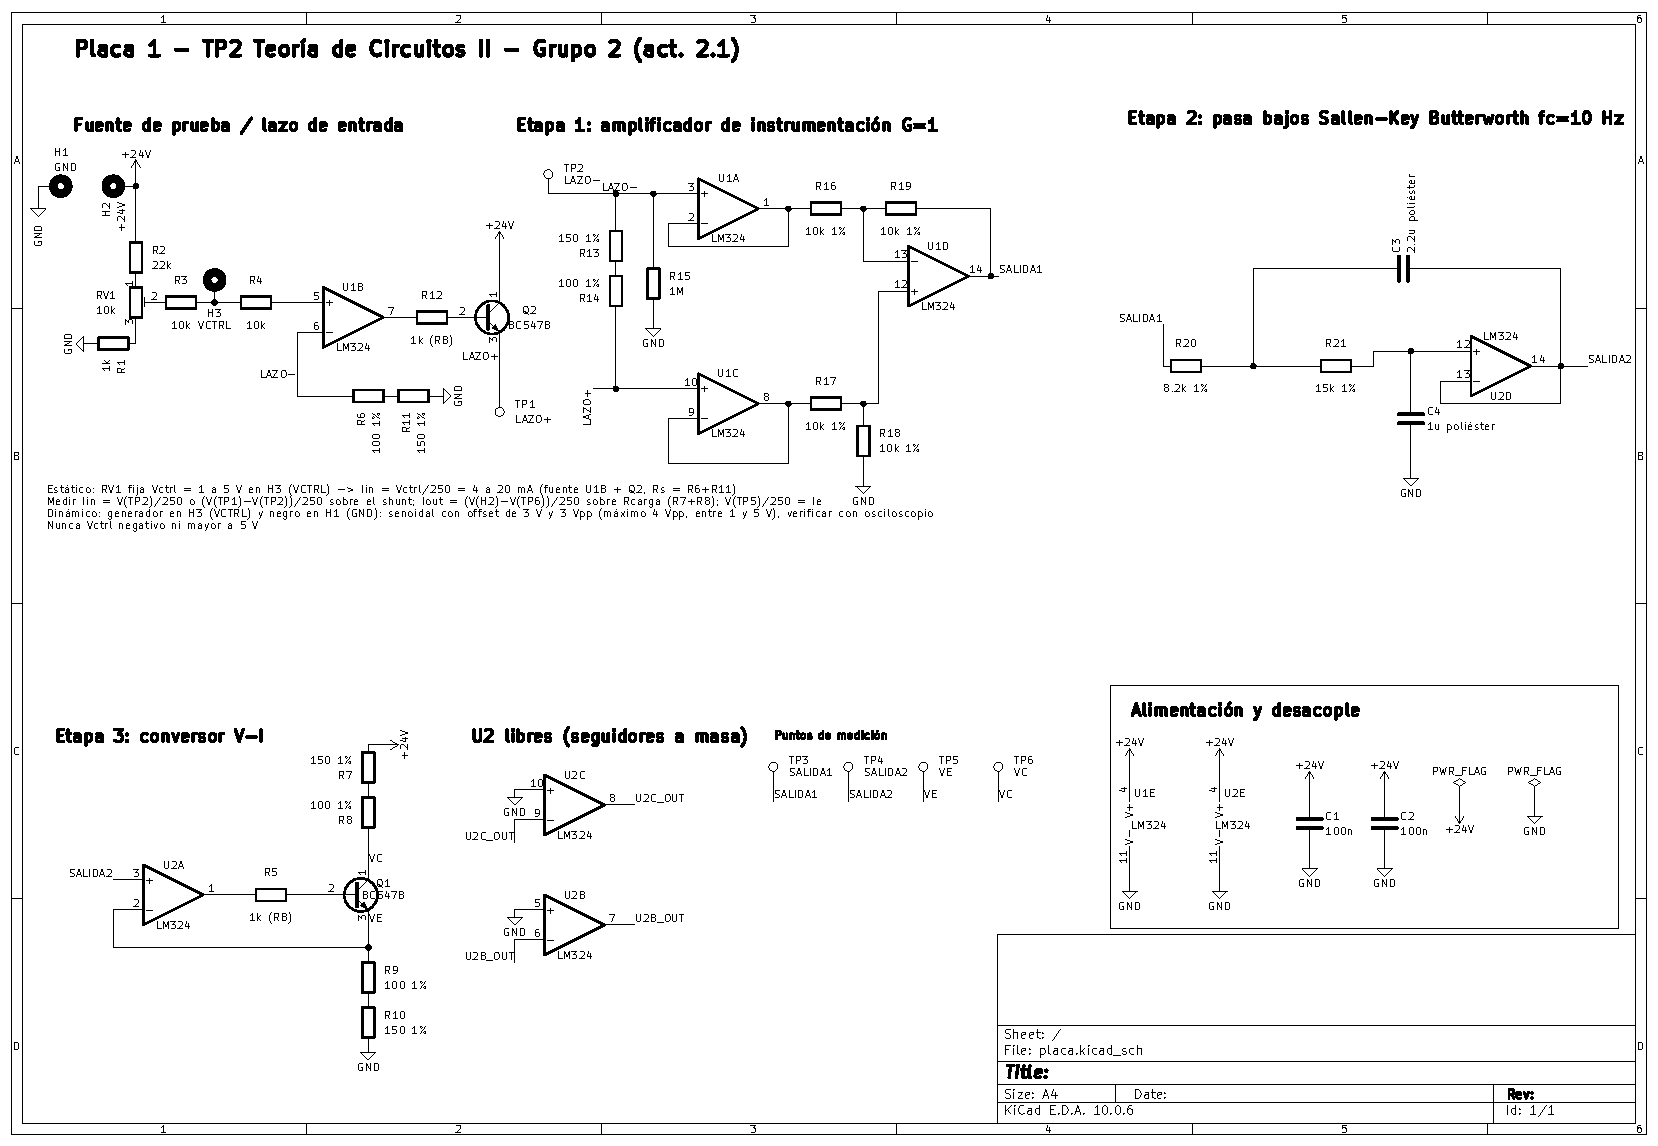
\includegraphics[angle=90,height=0.82\textheight]{images/fig_campo_kicad_esquematico.pdf}
  \caption{Esquemático en KiCad de la placa del filtro de señal de campo.}
  \label{crkt:anexo-campo-esquematico}
\end{figure}

\begin{figure}[H]
  \centering
  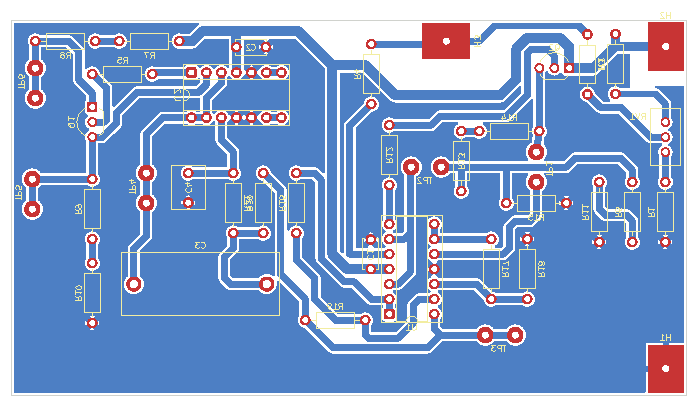
\includegraphics[width=\textwidth]{images/fig_campo_pcb_ruteo.pdf}
  \caption{Ruteo de la placa del filtro de señal de campo, espejado: capa inferior B.Cu (azul) y serigrafía
    (amarillo).}
  \label{fig:anexo-campo-pcb-ruteo}
\end{figure}

\begin{figure}[H]
  \centering
  \begin{subfigure}[t]{0.49\textwidth}
    \centering
    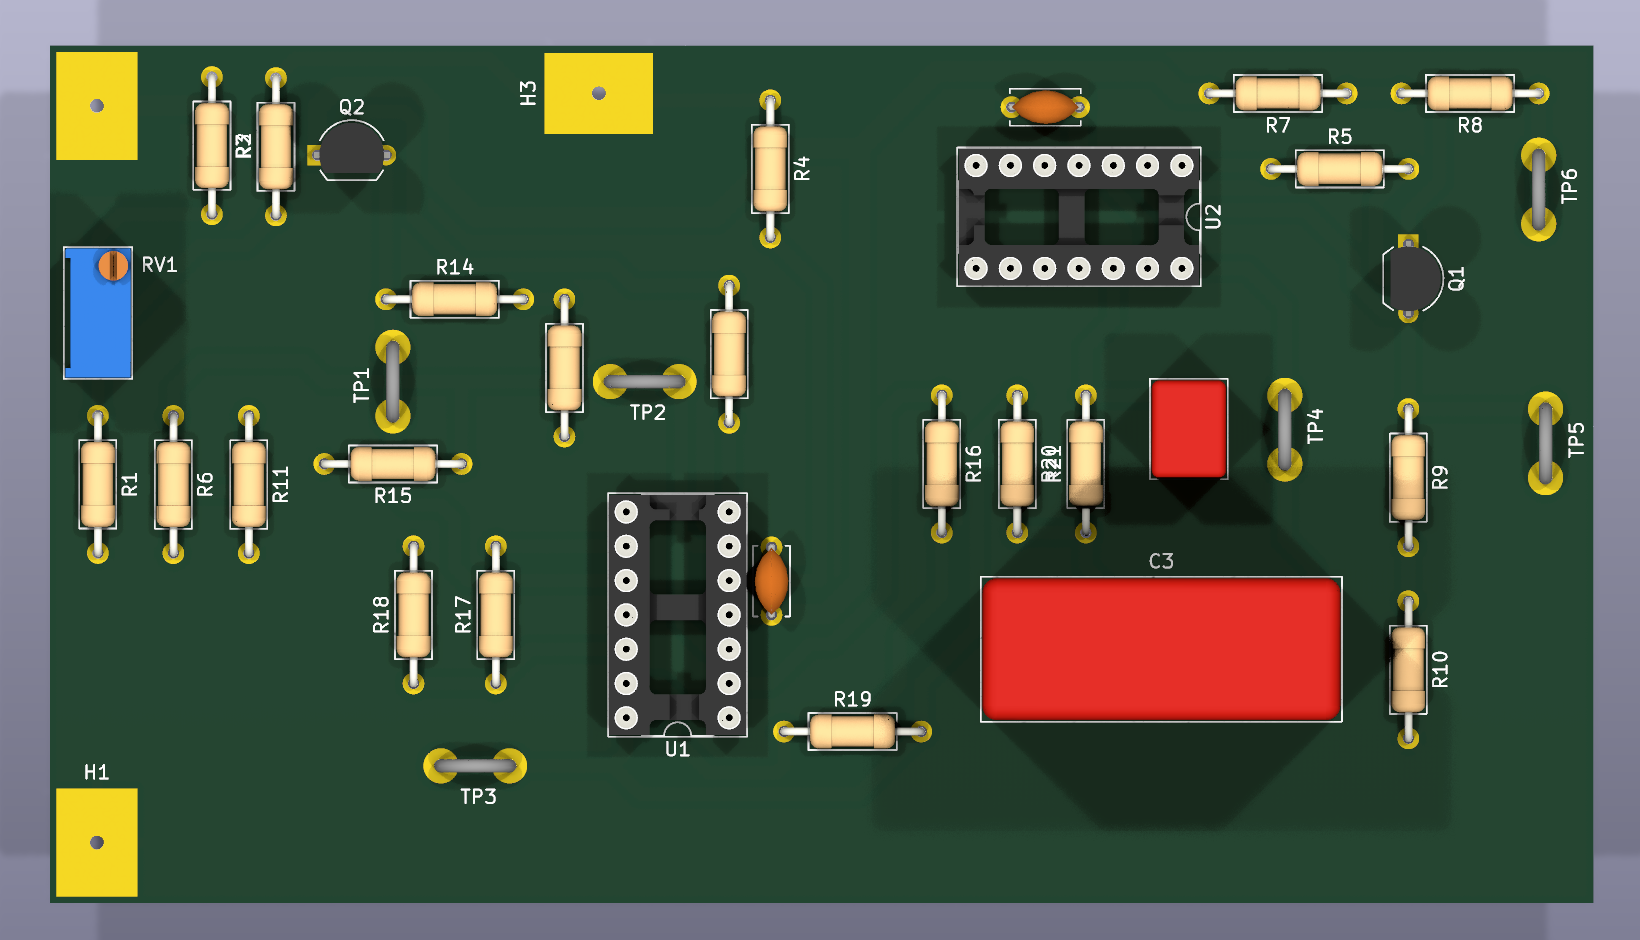
\includegraphics[width=\textwidth]{images/fig_campo_3d_top.png}
    \caption{Vista superior.}
    \label{fig:anexo-campo-3d-top}
  \end{subfigure}
  \hfill
  \begin{subfigure}[t]{0.49\textwidth}
    \centering
    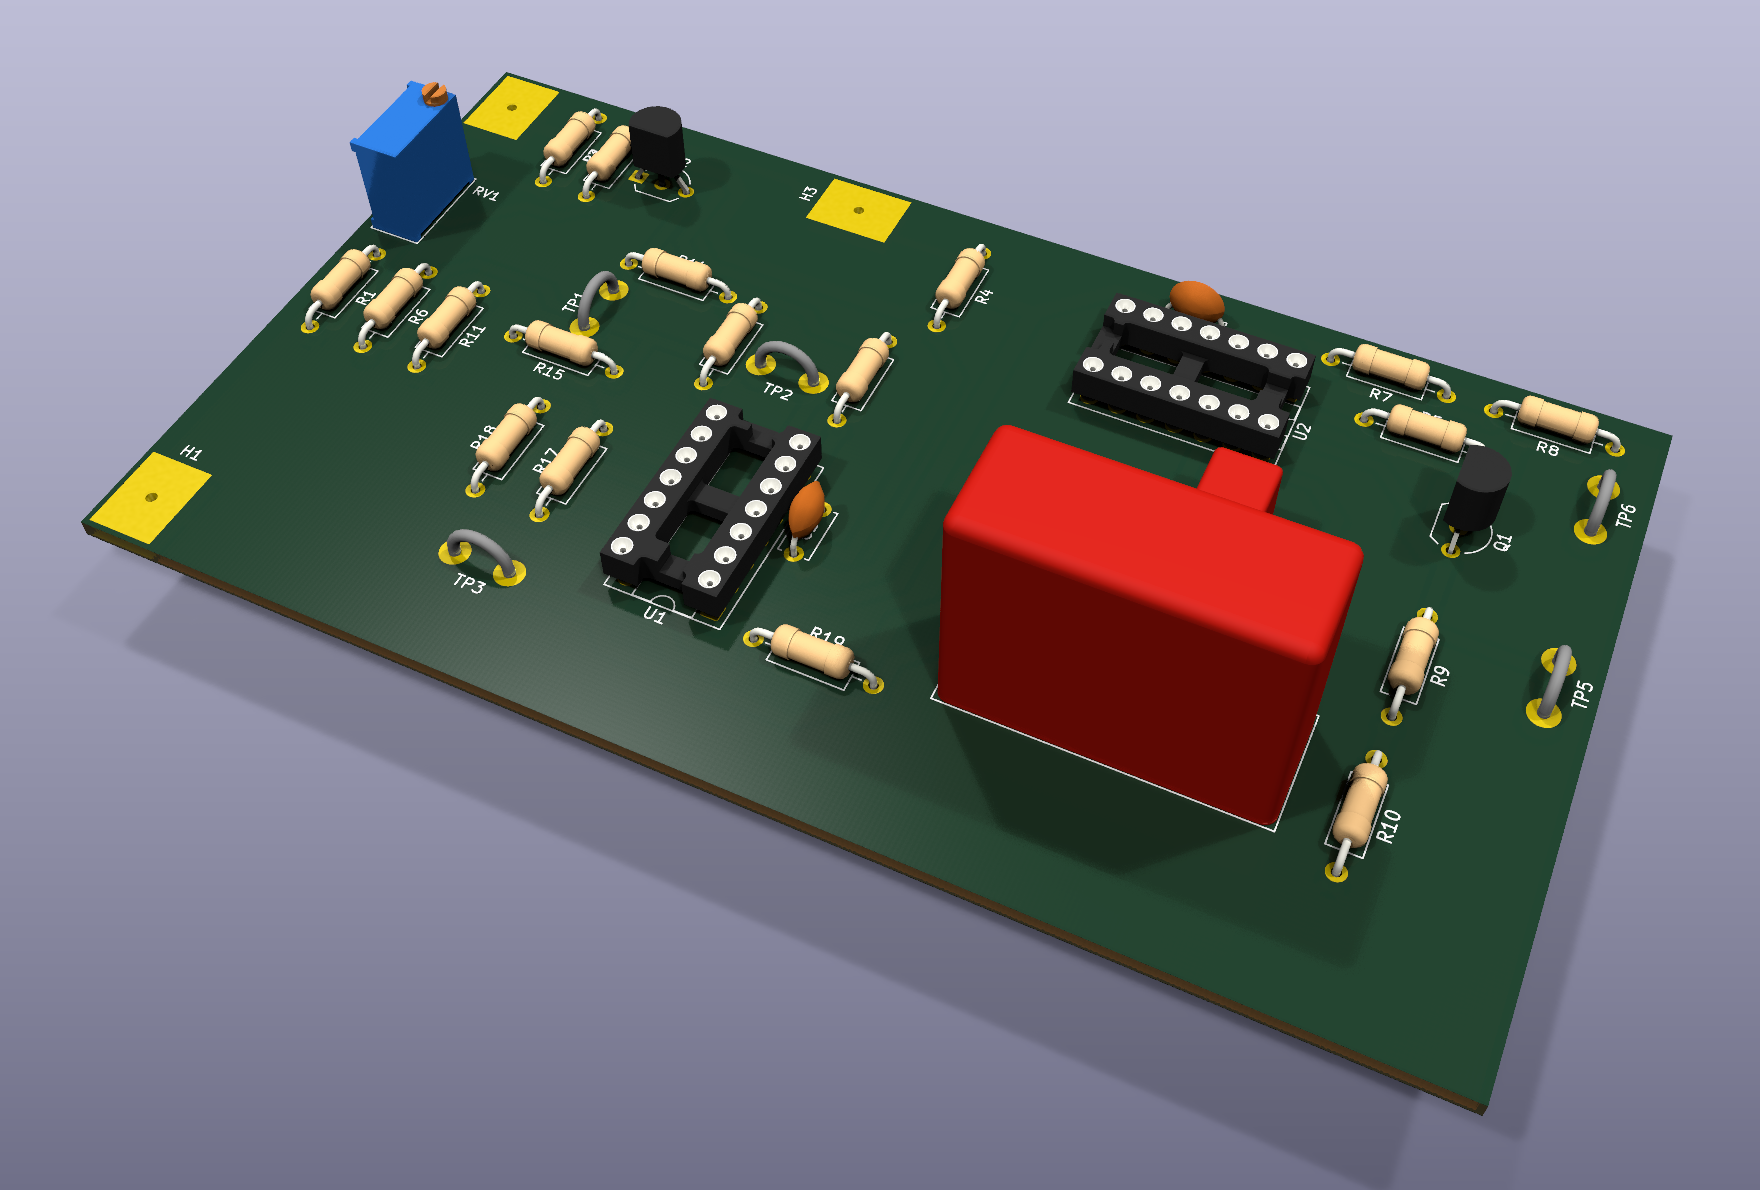
\includegraphics[width=\textwidth]{images/fig_campo_3d_iso.png}
    \caption{Vista isométrica.}
    \label{fig:anexo-campo-3d-iso}
  \end{subfigure}
  \caption{Vista 3D en KiCad de la placa del filtro de señal de campo.}
  \label{fig:anexo-campo-3d}
\end{figure}

\begin{figure}[H]
  \centering
  \begin{subfigure}[t]{0.49\textwidth}
    \centering
    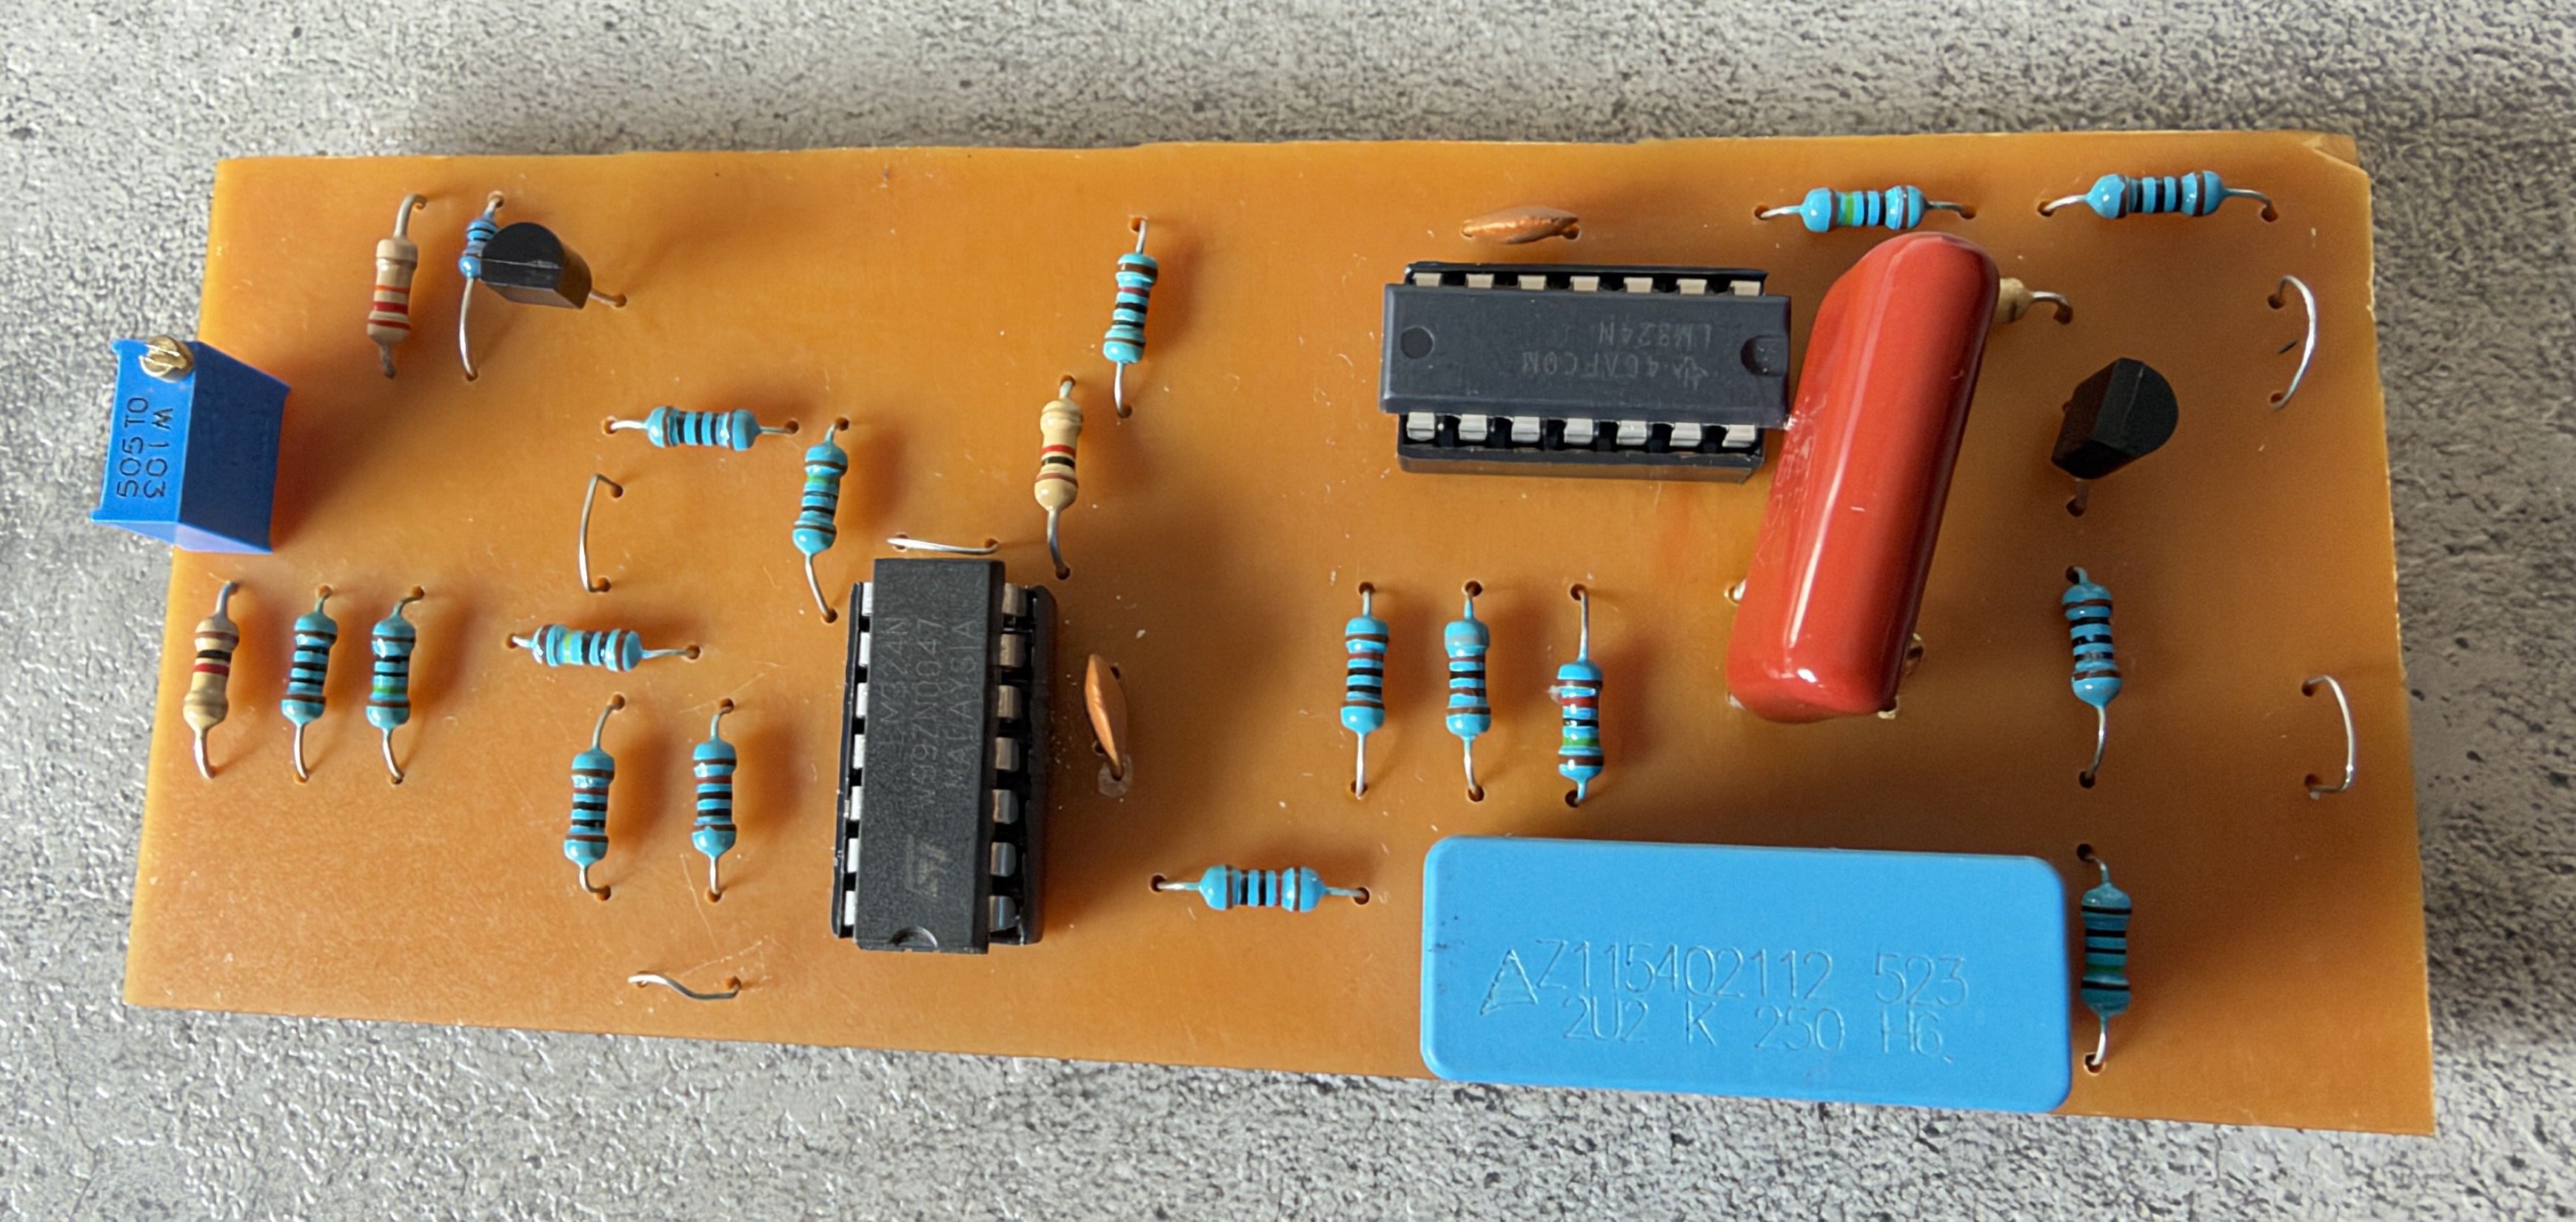
\includegraphics[width=\textwidth]{pictures/img_placa_campo_arriba.jpeg}
    \caption{Vista superior.}
    \label{fig:anexo-campo-fotos-arriba}
  \end{subfigure}
  \hfill
  \begin{subfigure}[t]{0.49\textwidth}
    \centering
    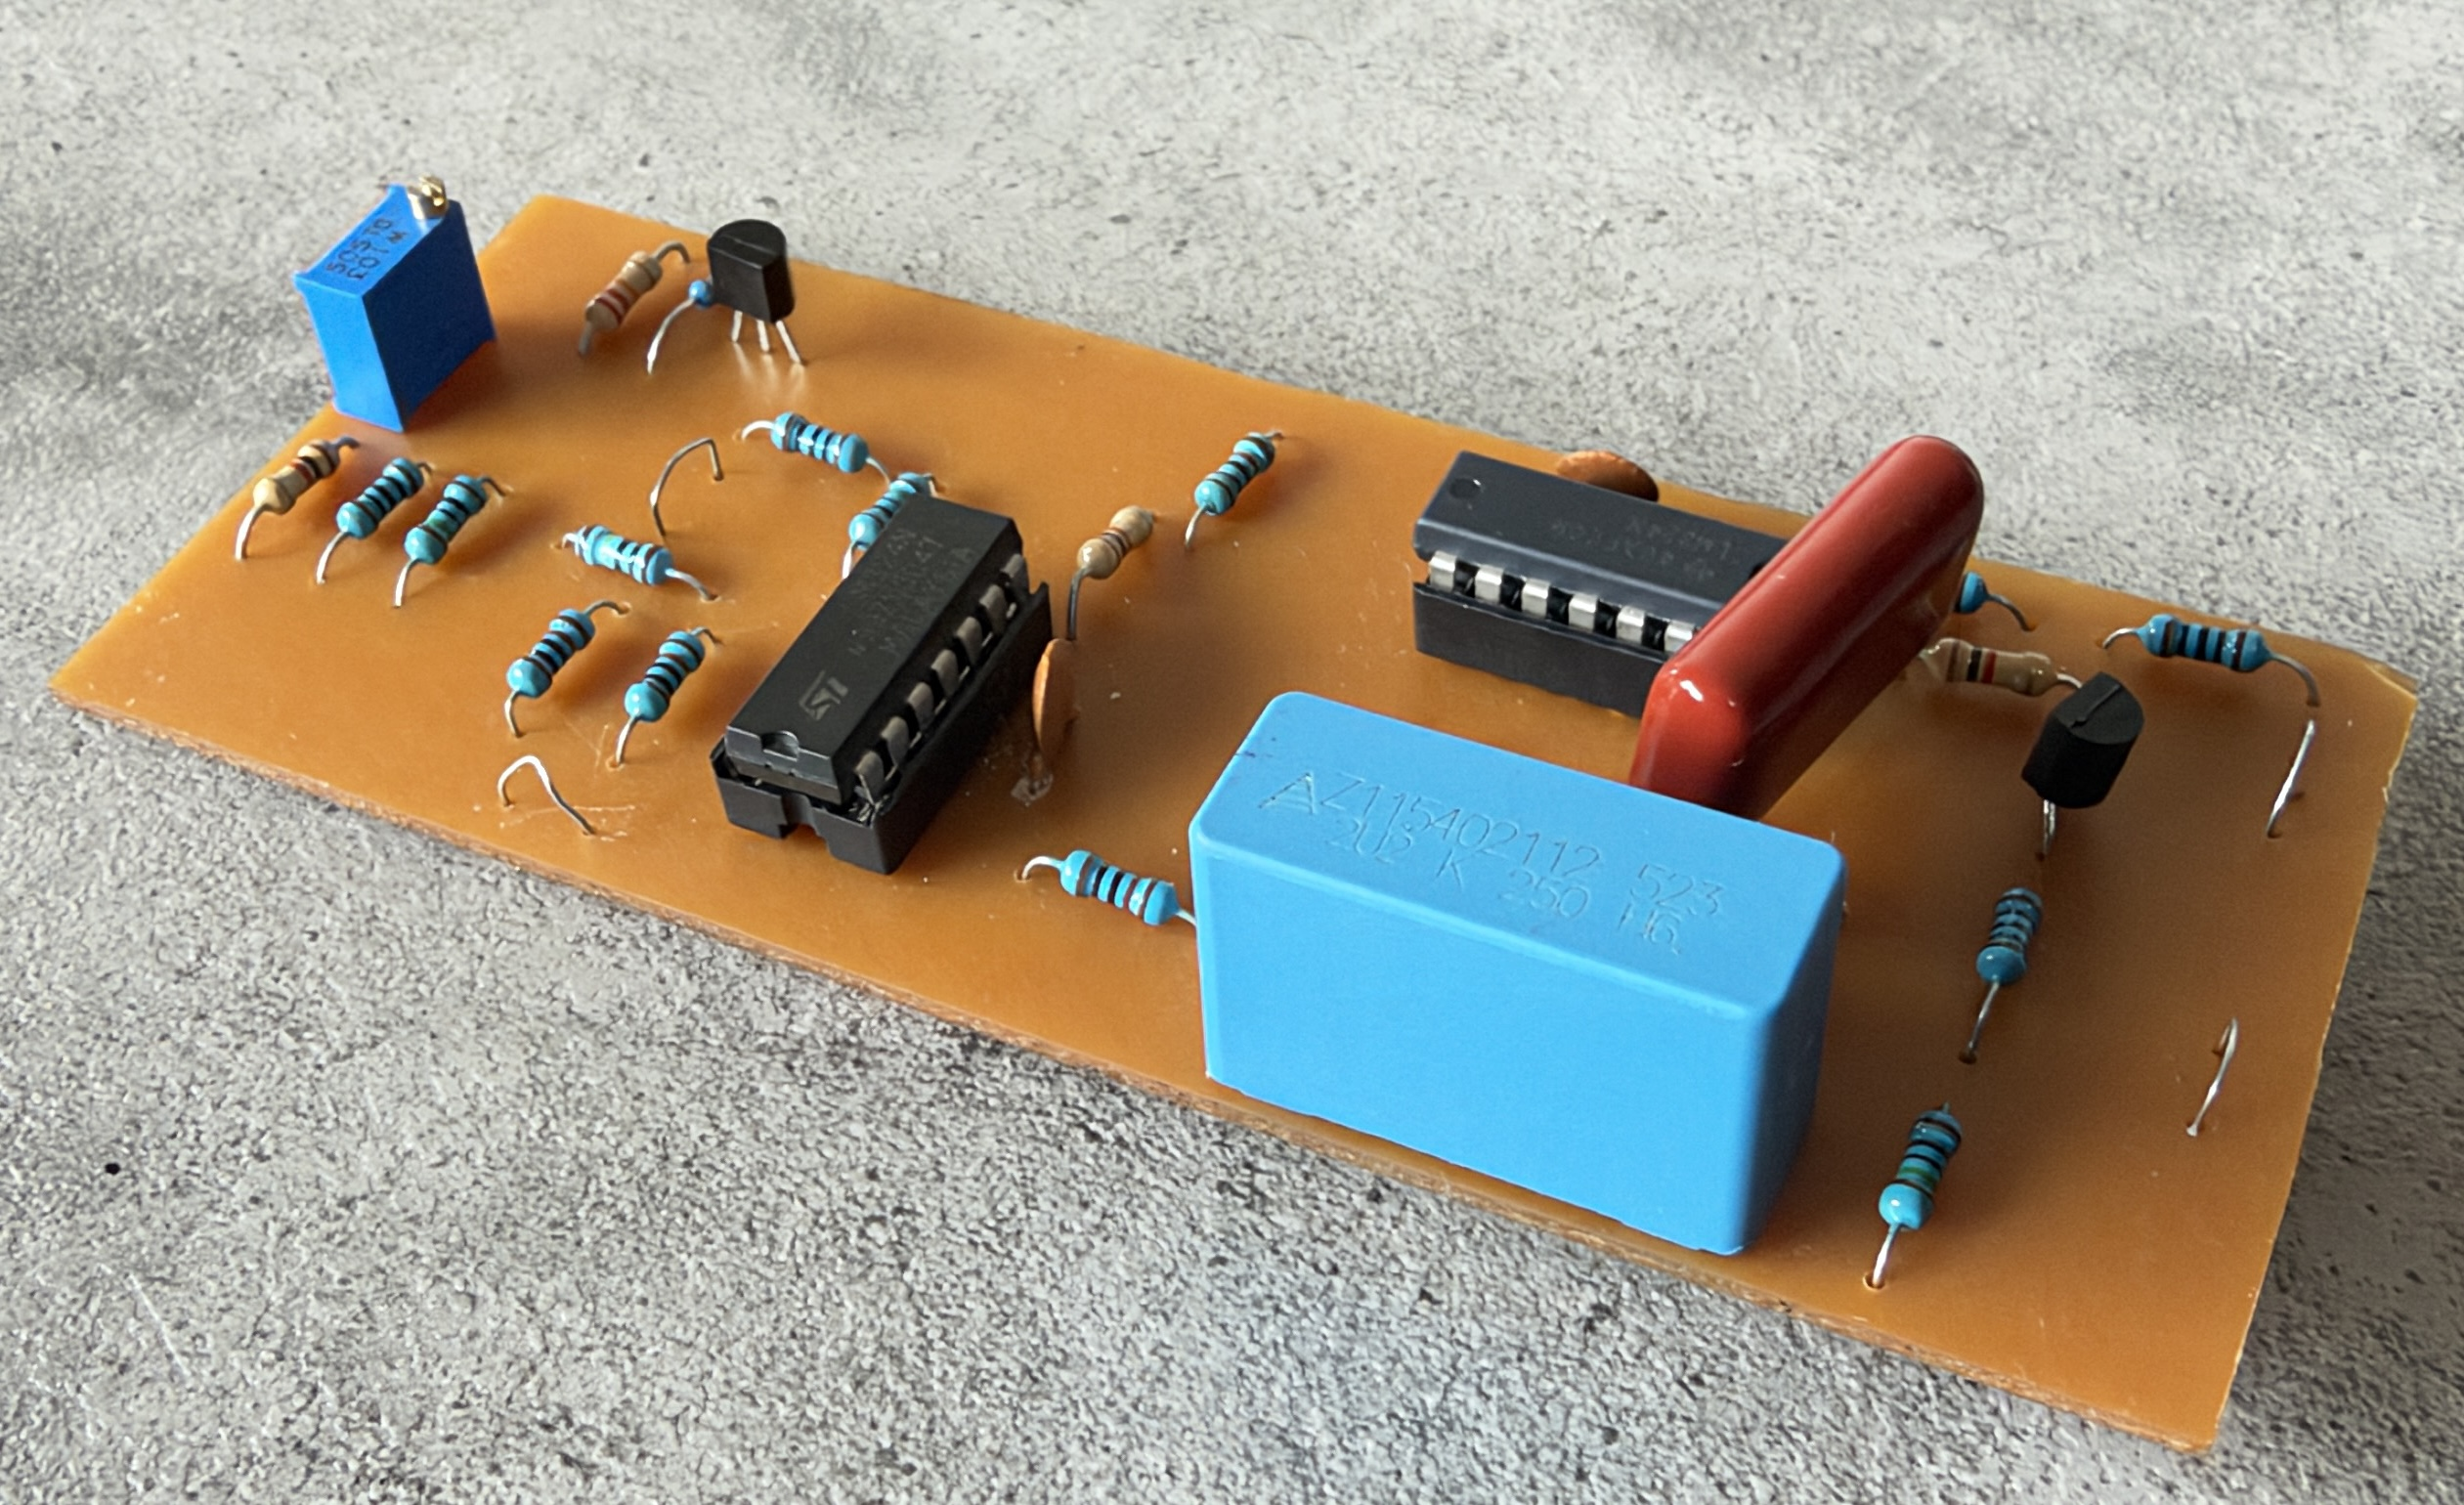
\includegraphics[width=\textwidth]{pictures/img_placa_campo_iso.jpeg}
    \caption{Vista isométrica.}
    \label{fig:anexo-campo-fotos-iso}
  \end{subfigure}
  \caption{Fotografías de la placa del filtro de señal de campo construida.}
  \label{fig:anexo-campo-fotos}
\end{figure}

\chapter{Placa de los filtros pasa bajos y pasa altos}
\label{chap:anexo-pcb}

\begin{figure}[H]
  \centering
  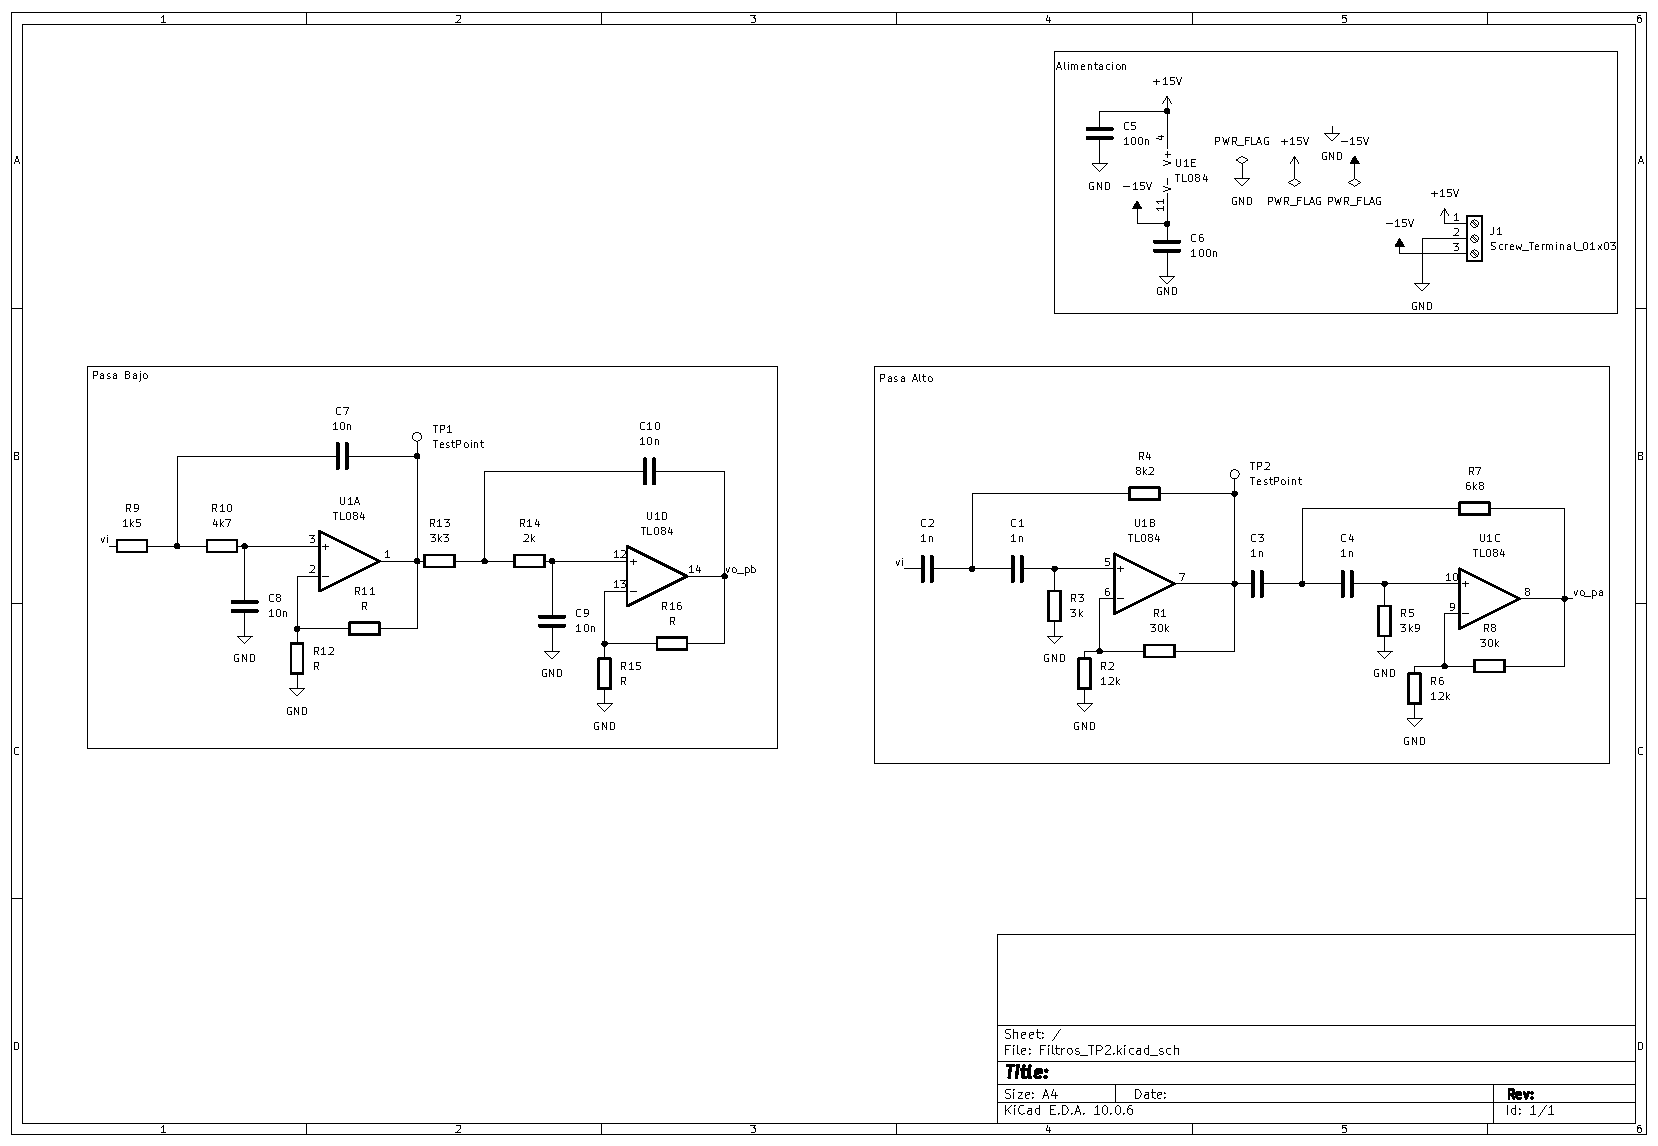
\includegraphics[angle=90,height=0.82\textheight]{images/fig_filtros_kicad_esquematico.pdf}
  \caption{Esquemático en KiCad de la placa de filtros: pasa bajos (izquierda), pasa altos (derecha) y alimentación
    del TL084 (arriba).}
  \label{crkt:anexo-filtros-esquematico}
\end{figure}

\begin{table}[!ht]
  \centering
  \begin{tabular}{|l|c|c|c|}
    \hline
    Filtro & Informe & KiCad & Valor \\
    \hline
    \multirow{8}{*}{Pasa bajos} & $R_1$ & R9 & $\SI{1.5}{\kilo\ohm}$ \\
    & $R_2$ & R10 & $\SI{4.7}{\kilo\ohm}$ \\
    & $R_3$ & R13 & $\SI{3.3}{\kilo\ohm}$ \\
    & $R_4$ & R14 & $\SI{2.0}{\kilo\ohm}$ \\
    & $R_{a1}$ / $R_{b1}$ & R12 / R11 & $\SI{10}{\kilo\ohm}$ \\
    & $R_{a2}$ / $R_{b2}$ & R15 / R16 & $\SI{10}{\kilo\ohm}$ \\
    & $C_1$, $C_2$ (celda 1) & C7, C8 & $\SI{10}{\nano\farad}$ \\
    & $C_3$, $C_4$ (celda 2) & C9, C10 & $\SI{10}{\nano\farad}$ \\
    \hline
    \multirow{8}{*}{Pasa altos} & $R_1$ (a masa) & R3 & $\SI{3.0}{\kilo\ohm}$ \\
    & $R_2$ (realim.) & R4 & $\SI{8.2}{\kilo\ohm}$ \\
    & $R_3$ (a masa) & R5 & $\SI{3.9}{\kilo\ohm}$ \\
    & $R_4$ (realim.) & R7 & $\SI{6.8}{\kilo\ohm}$ \\
    & $R_{a1}$ / $R_{b1}$ & R2 / R1 & $\SI{12}{\kilo\ohm}$ / $\SI{30}{\kilo\ohm}$ \\
    & $R_{a2}$ / $R_{b2}$ & R6 / R8 & $\SI{12}{\kilo\ohm}$ / $\SI{30}{\kilo\ohm}$ \\
    & $C_1$, $C_2$ (celda 1) & C2, C1 & $\SI{1}{\nano\farad}$ \\
    & $C_3$, $C_4$ (celda 2) & C3, C4 & $\SI{1}{\nano\farad}$ \\
    \hline
    \multirow{2}{*}{Común} & Desacople & C5, C6 & $\SI{100}{\nano\farad}$ \\
    & Operacional & U1 & TL084 \\
    \hline
  \end{tabular}
  \caption{Correspondencia entre la designación de componentes del informe y la del esquemático de KiCad.}
  \label{tab:anexo-designadores}
\end{table}

\begin{figure}[H]
  \centering
  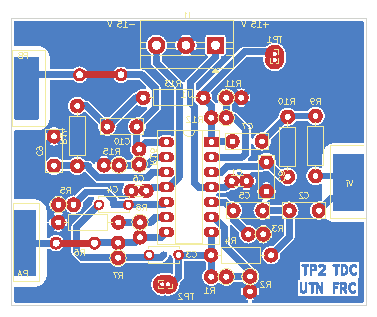
\includegraphics[width=0.8\textwidth]{images/fig_filtros_pcb_ruteo.pdf}
  \caption{Ruteo de la placa de filtros, espejado: capa inferior B.Cu (azul), puentes en F.Cu (rojo) y serigrafía
    (amarillo).}
  \label{fig:anexo-filtros-pcb-ruteo}
\end{figure}

\begin{figure}[H]
  \centering
  \begin{subfigure}[t]{0.49\textwidth}
    \centering
    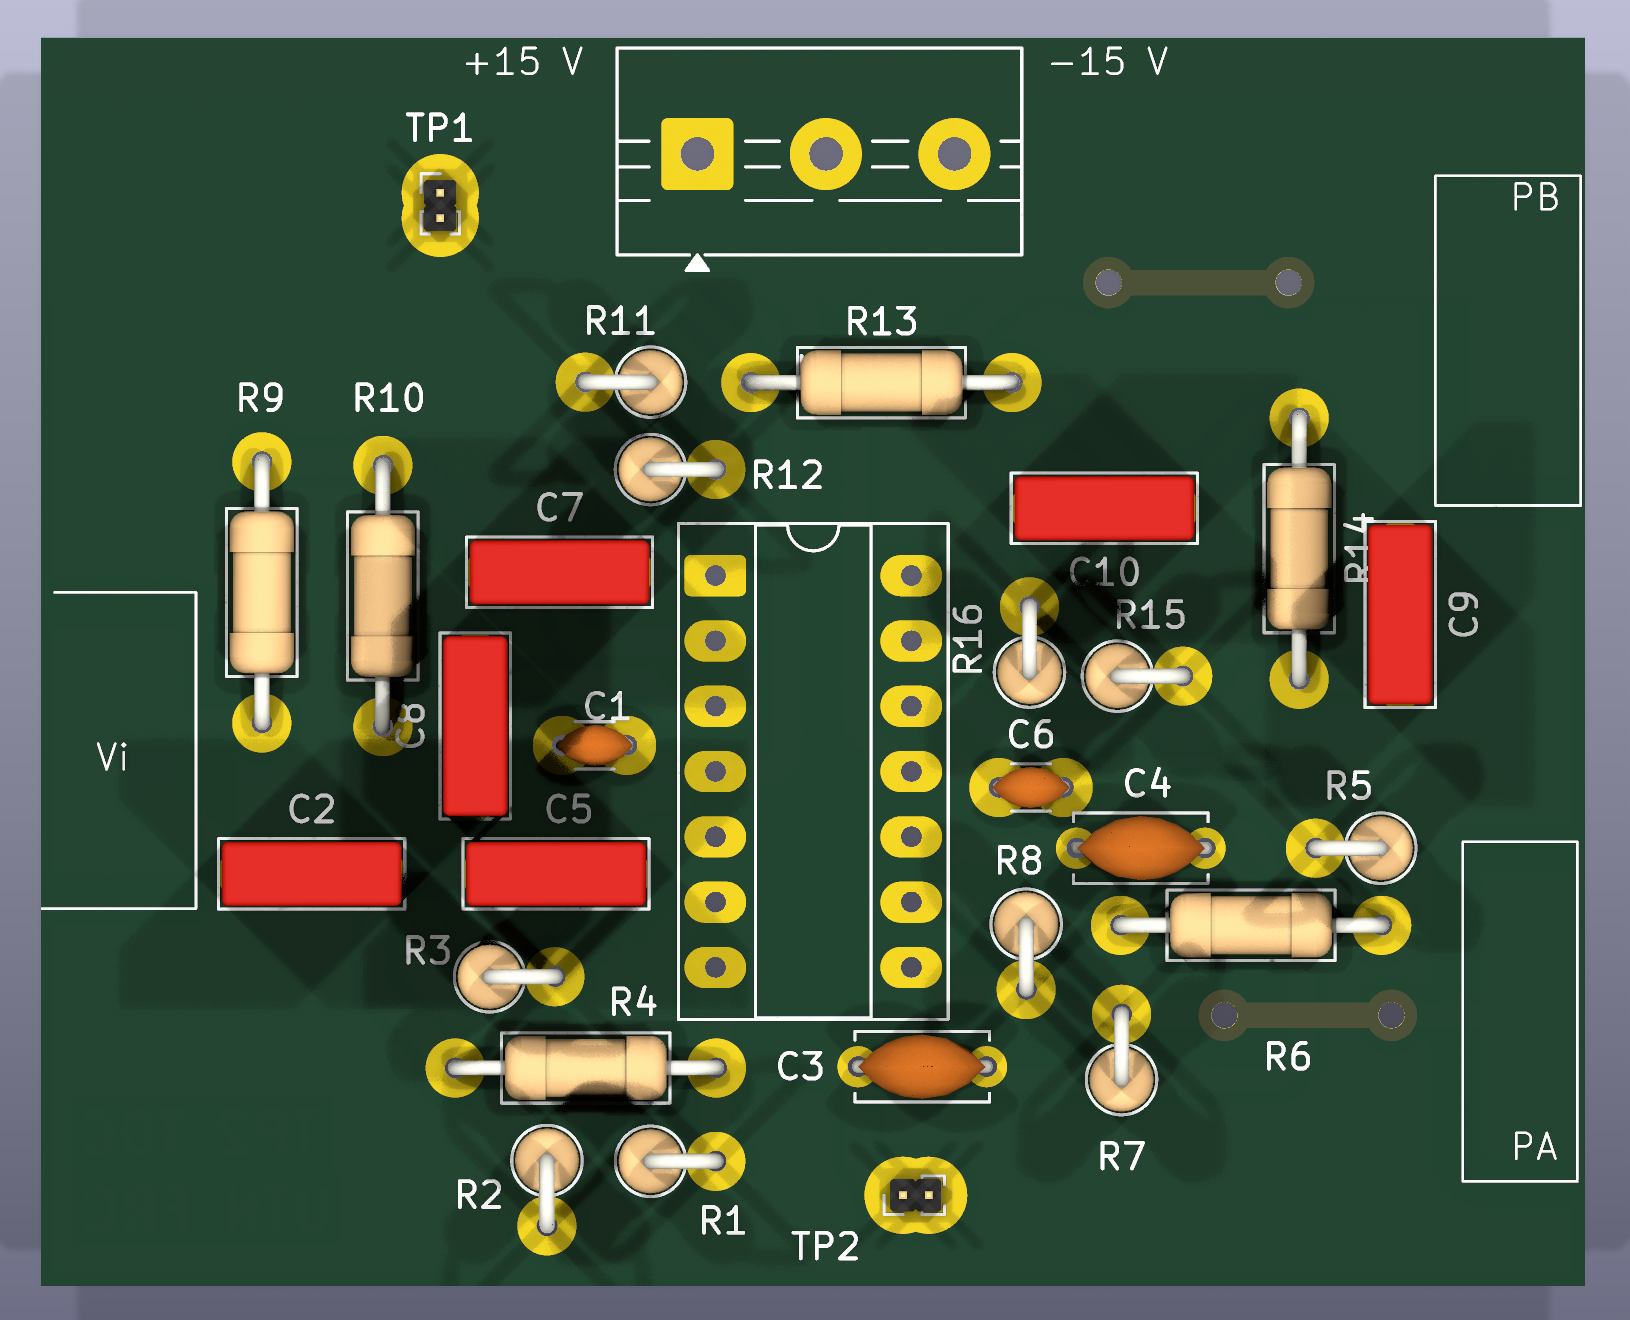
\includegraphics[width=\textwidth]{images/fig_filtros_3d_top.png}
    \caption{Vista superior.}
    \label{fig:anexo-filtros-3d-top}
  \end{subfigure}
  \hfill
  \begin{subfigure}[t]{0.49\textwidth}
    \centering
    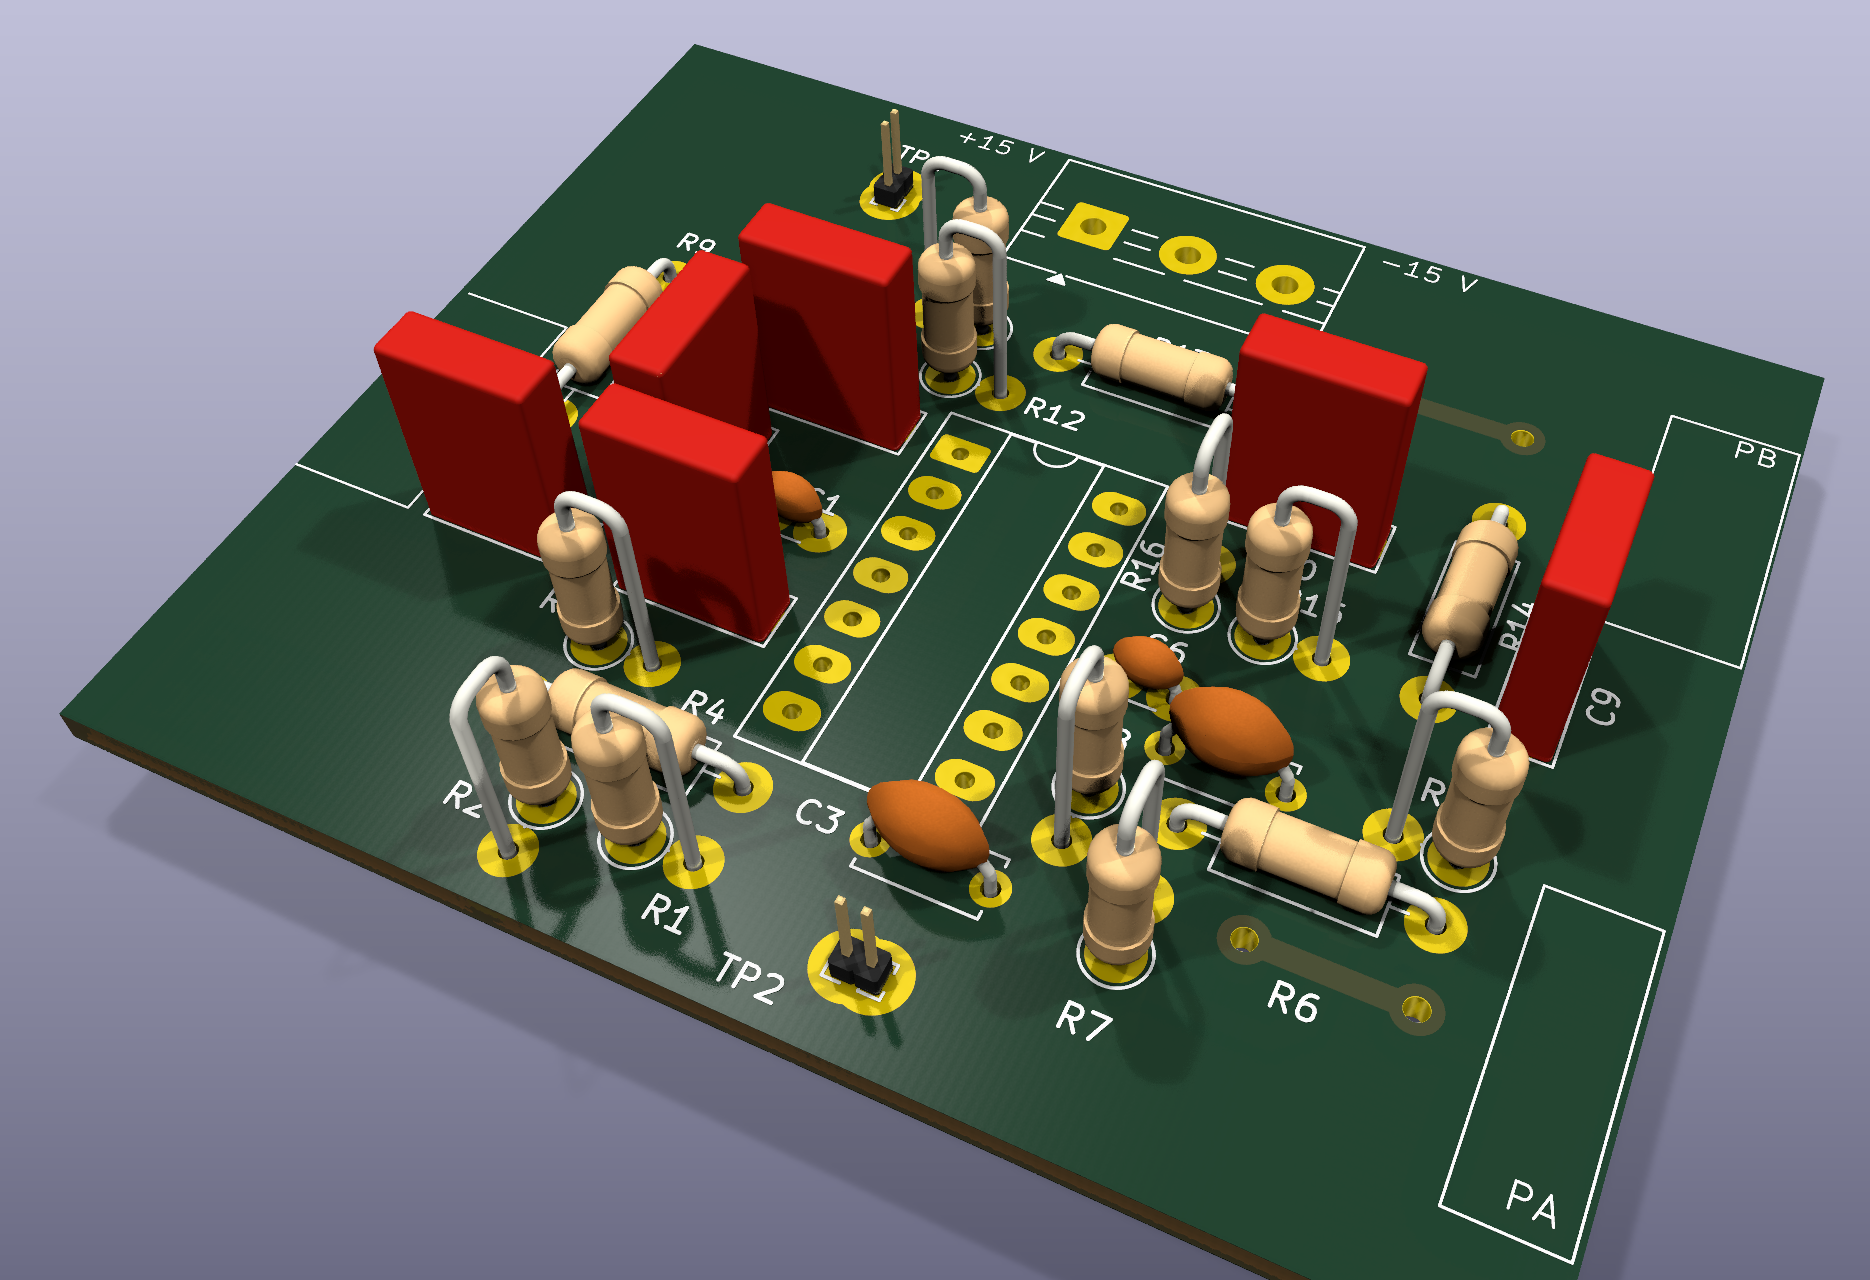
\includegraphics[width=\textwidth]{images/fig_filtros_3d_iso.png}
    \caption{Vista isométrica.}
    \label{fig:anexo-filtros-3d-iso}
  \end{subfigure}
  \caption{Vista 3D en KiCad de la placa de los filtros pasa bajos y pasa altos.}
  \label{fig:anexo-filtros-3d}
\end{figure}

\begin{figure}[H]
  \centering
  \begin{subfigure}[t]{0.49\textwidth}
    \centering
    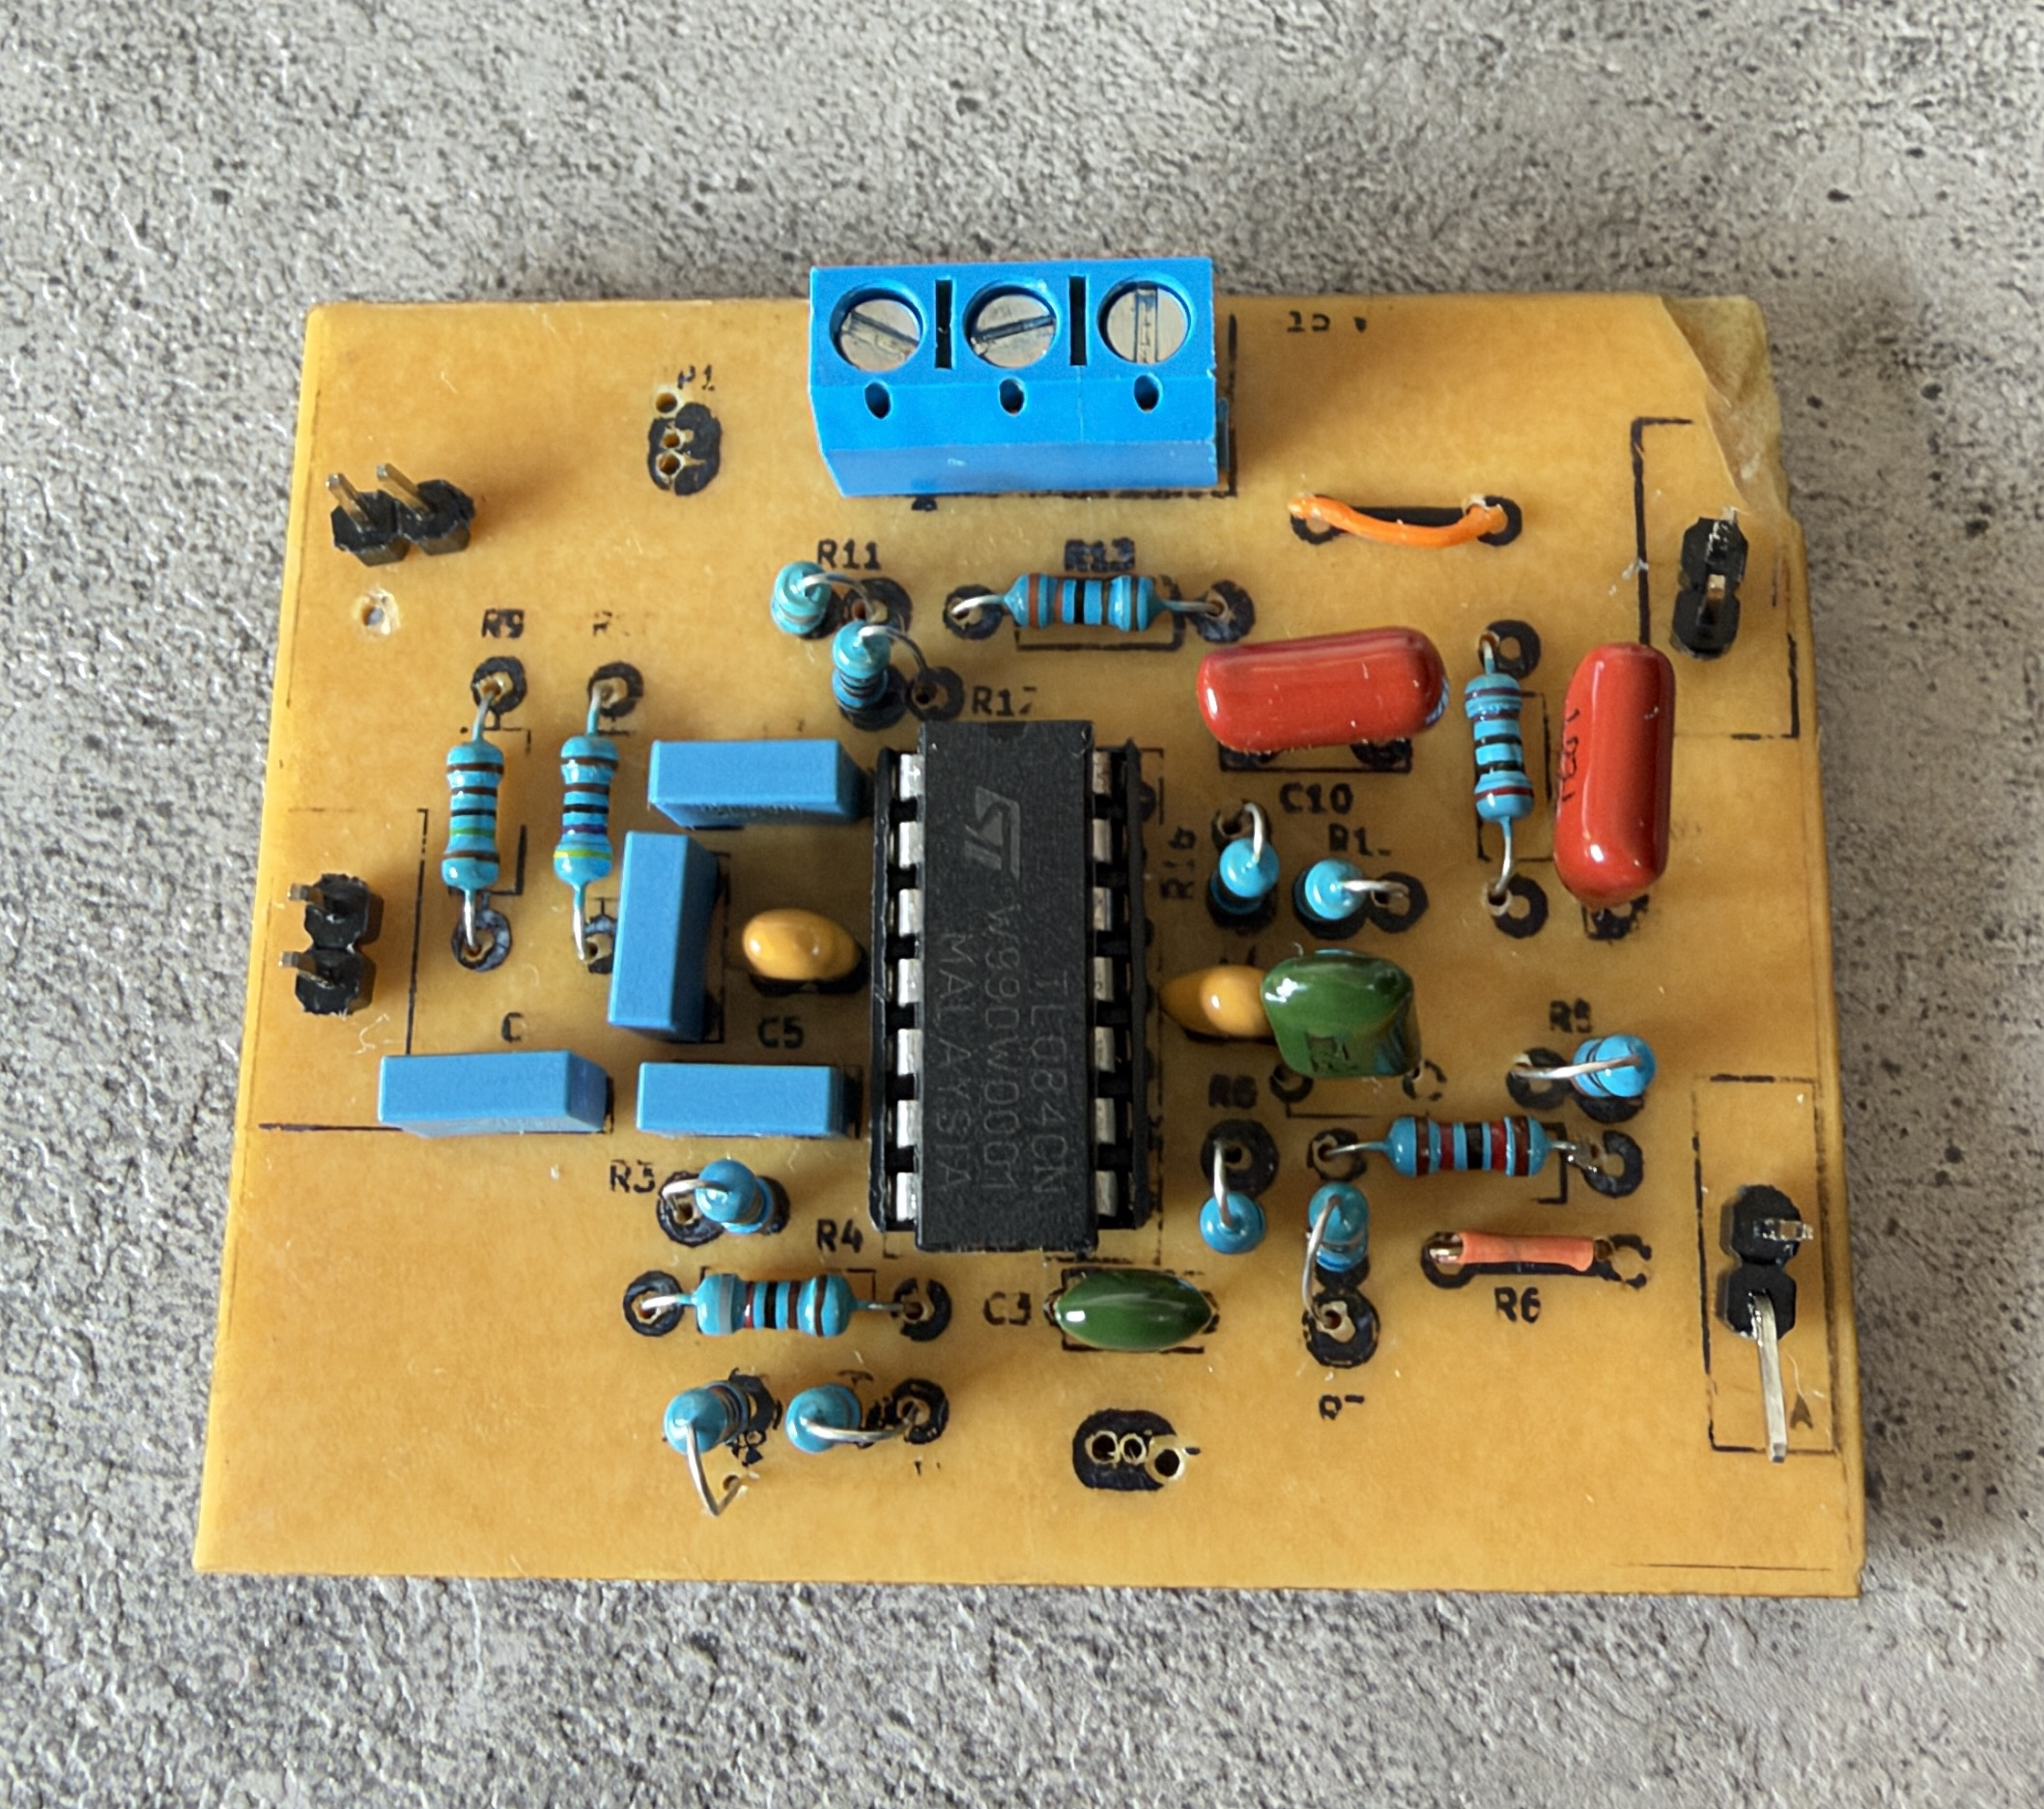
\includegraphics[width=\textwidth]{pictures/img_placa_filtros_arriba.jpeg}
    \caption{Vista superior.}
    \label{fig:anexo-filtros-fotos-arriba}
  \end{subfigure}
  \hfill
  \begin{subfigure}[t]{0.49\textwidth}
    \centering
    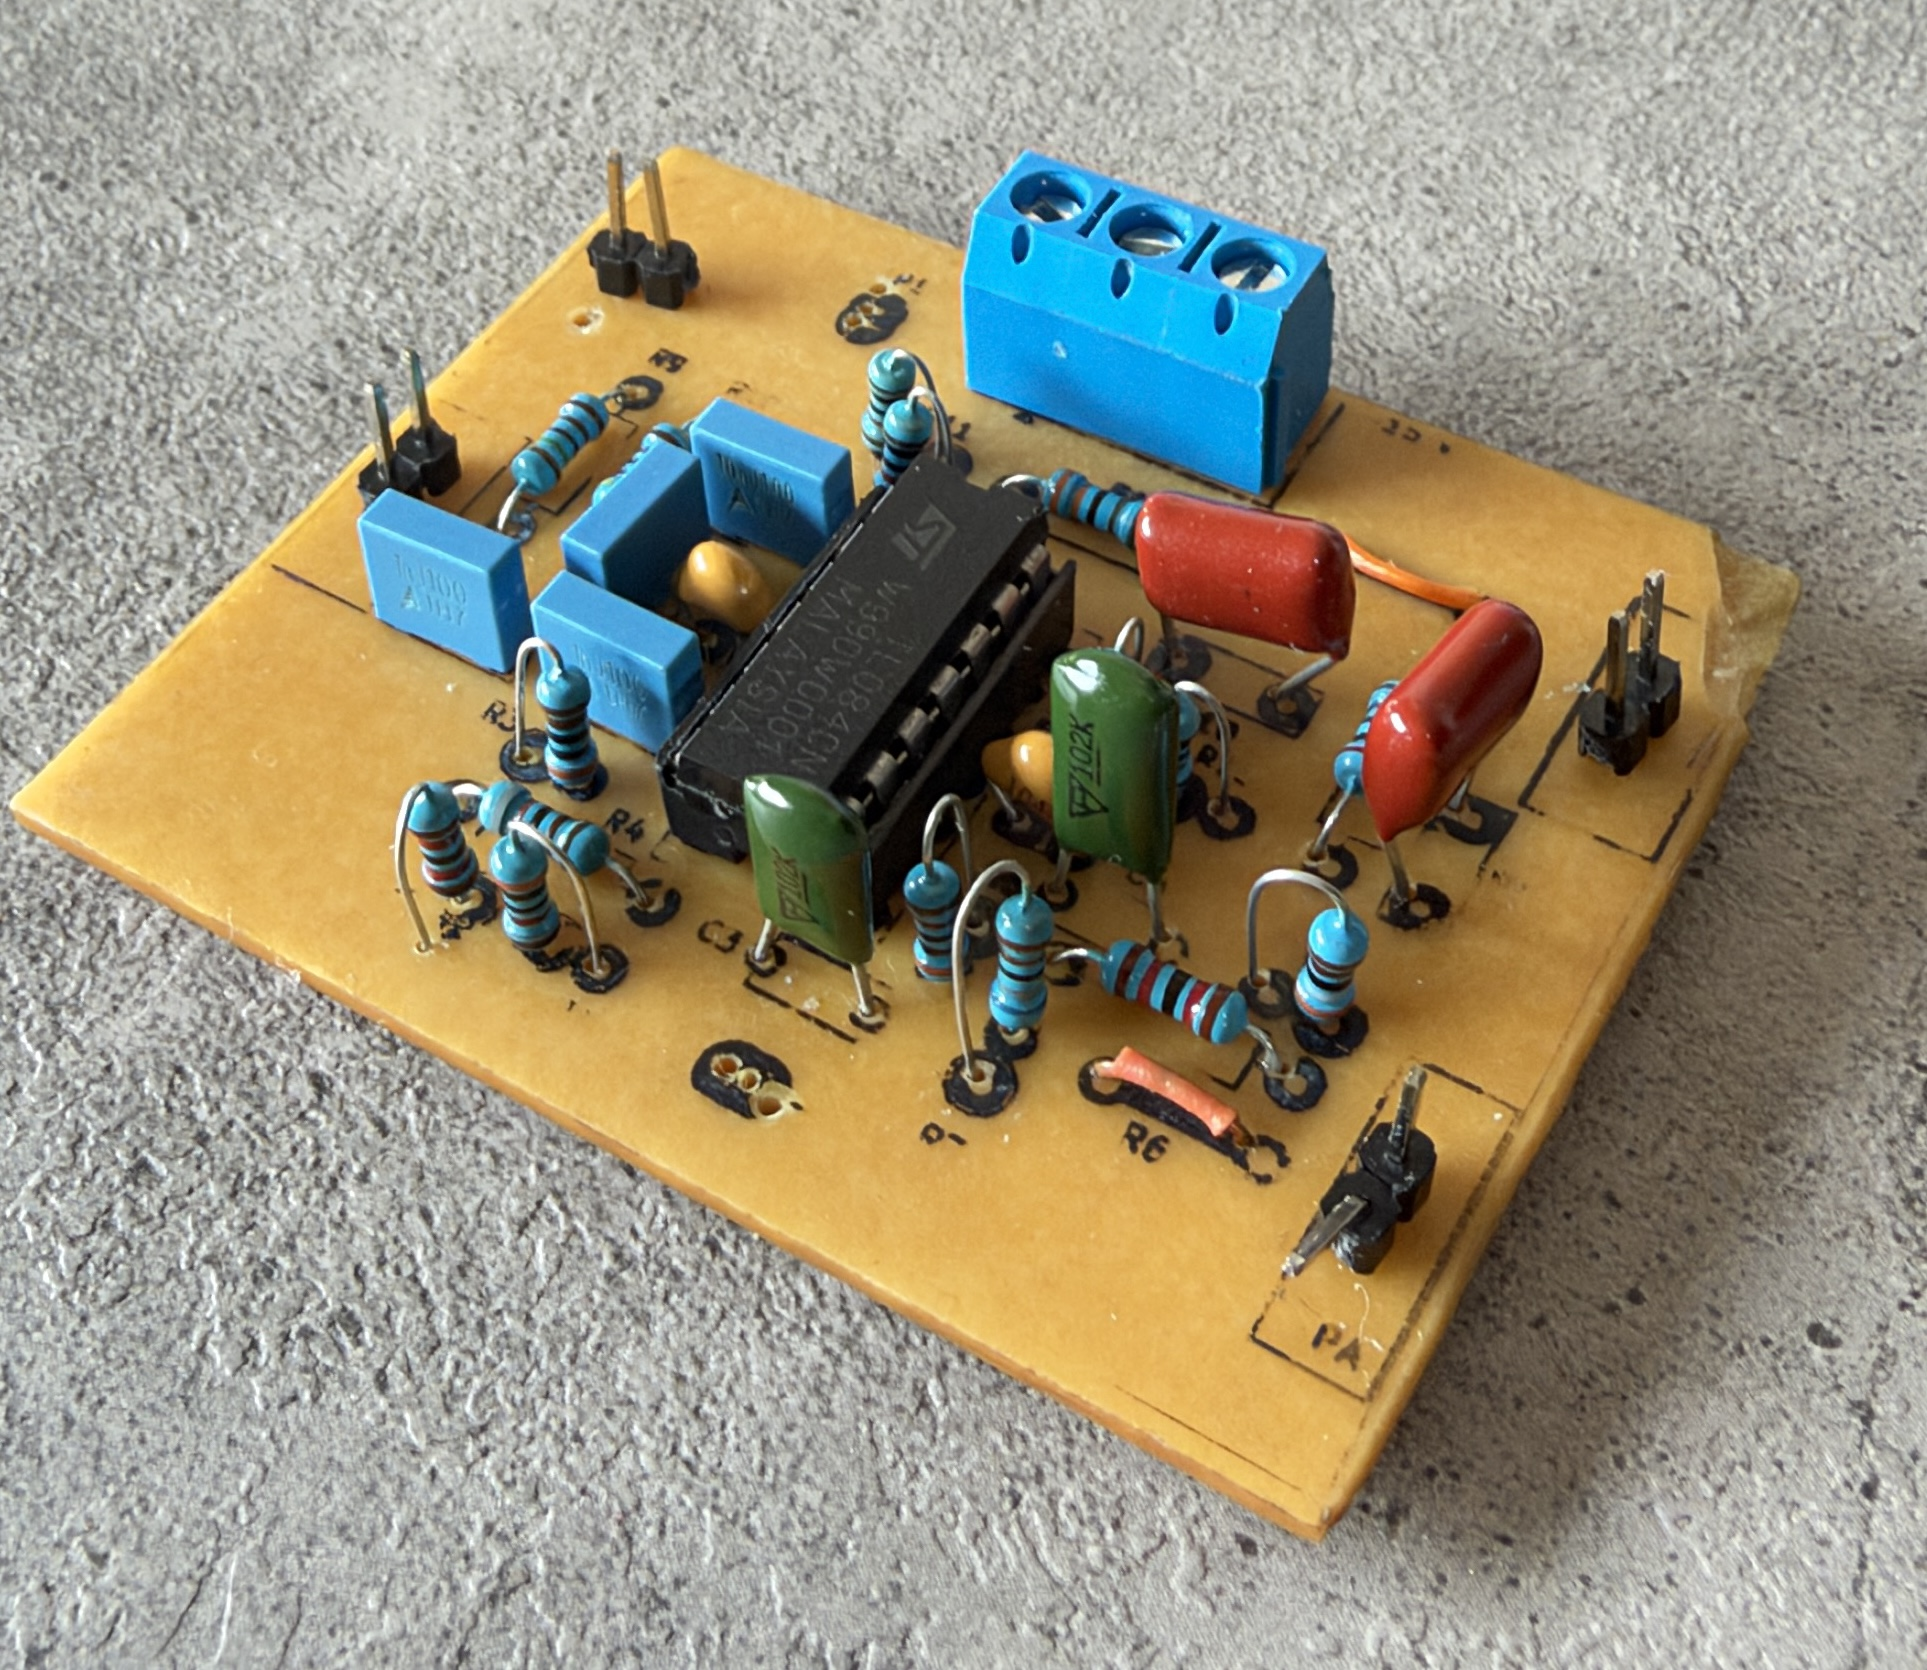
\includegraphics[width=\textwidth]{pictures/img_placa_filtros_iso.jpeg}
    \caption{Vista isométrica.}
    \label{fig:anexo-filtros-fotos-iso}
  \end{subfigure}
  \caption{Fotografías de la placa de los filtros pasa bajos y pasa altos construida.}
  \label{fig:anexo-filtros-fotos}
\end{figure}

\chapter{Lista de materiales (BOM) y balance de compras}
\label{chap:anexo-bom}

A fin de coordinar la fabricación y el montaje de las placas del grupo, se detalla el balance consolidado entre
componentes disponibles en stock y componentes adquiridos para el laboratorio.

\section{Placa 1: Receptor y filtro de señal de campo
  \texorpdfstring{$\SI{4}{}$--$\SI{20}{\milli\ampere}$}{4--20 mA}}
\label{sec:anexo-bom-placa1}

\begin{table}[!ht]
  \centering
  \resizebox{\textwidth}{!}{%
  \begin{tabular}{|l|c|c|c|p{7cm}|}
    \hline
    Componente / Valor & Req. & Stock & A Comprar & Observaciones \\
    \hline
    Integrado LM324N & 2 & 2 & 0 & Cubierto (fuente simple $+\SI{24}{\volt}$). \\
    Zócalo DIP-14 & 2 & 2 & 0 & Cubierto. \\
    Transistor NPN BC337 & 1 & 0 & 2 & Sumidero etapa 3
      ($V_{CE}\approx \SI{14}{\volt}, P_D\approx \SI{0.28}{\watt}$). \\
    Resistores $\SI{250}{\ohm}$ ($\SI{1}{\percent}$) & 3 & 0 & 5 & Shunt de entrada, salida y carga. \\
    Resistores $\SI{10}{\kilo\ohm}$ ($\SI{1}{\percent}$) & 4 & 0 & 6
      & Críticos para el CMRR del receptor diferencial. \\
    Resistores $\SI{1}{\mega\ohm}$ y $\SI{1}{\kilo\ohm}$ & 1 + 1 & 0 & 2 + 2
      & Polarización modo común y base del transistor. \\
    Capacitores filtro $\SI{10}{\hertz}$ ($\SI{1}{\micro\farad}$ y $\SI{2.2}{\micro\farad}$) & 1 + 1 & 1 + 1 & 0
      & Poliéster $>\SI{63}{\volt}$ cubiertos. \\
    Resistores filtro $\SI{10}{\hertz}$ ($\approx\SI{11}{\kilo\ohm}$) & 2 & 0 & 4 & Para $f_c = \SI{10}{\hertz}$. \\
    Desacople $\SI{100}{\nano\farad}$ cerámico & 2 & 2 & 0 & Pegados a pines 4 y 11 del LM324. \\
    Borneras 2 pines + Pin Headers & 3 + 1 tira & 0 & 4 + 1 tira
      & Conexiones de alimentación, lazo y test points. \\
    \hline
  \end{tabular}%
  }
  \caption{Lista de materiales para Placa 1 (Señal de campo).}
  \label{tab:bom-placa1}
\end{table}

\section{Placa 2: Filtro Pasa Bajos y Filtro Pasa Altos (Orden 4)}
\label{sec:anexo-bom-placa2}

\begin{table}[!ht]
  \centering
  \resizebox{\textwidth}{!}{%
  \begin{tabular}{|l|c|c|c|p{7cm}|}
    \hline
    Componente / Valor & Req. & Stock & A Comprar & Asignación / Observaciones \\
    \hline
    Integrado TL084CN (DIP-14) & 1 ó 2 & 2 & 0 & Cubierto. \\
    Zócalos DIP-14 & 2 & 2 & 0 & Cubierto. \\
    Capacitores $\SI{1.0}{\nano\farad}$ (102) poliéster & 4 & 4 & 0
      & Cubiertos para Pasa Altos ($C_1\text{--}C_4$). \\
    Capacitor $\SI{10}{\nano\farad}$ (103) poliéster & 1 & 2 & 0 & Cubierto para Pasa Bajos Celda 2 ($C_4$). \\
    Capacitor $\SI{2.2}{\nano\farad}$ (222) poliéster & 1 & 0 & 3 & Pasa Bajos Celda 1 ($C_1$). \\
    Capacitores $\SI{3.3}{\nano\farad}$ (332) poliéster & 2 & 0 & 4
      & Pasa Bajos Celda 1 ($C_2$) y Celda 2 ($C_3$). \\
    Resistor $\SI{2.0}{\kilo\ohm}$ ($\SI{1}{\percent}$) & 1 & 0 & 3 & Pasa Bajos Celda 2 ($R_3$). \\
    Resistor $\SI{3.0}{\kilo\ohm}$ ($\SI{1}{\percent}$) & 1 & 0 & 3 & Pasa Altos Celda 1 ($R_1$). \\
    Resistores $\SI{3.9}{\kilo\ohm}$ ($\SI{1}{\percent}$) & 2 & 0 & 5
      & Pasa Bajos Celda 1 ($R_1$) + Pasa Altos Celda 2. \\
    Resistores $\SI{10}{\kilo\ohm}$ ($\SI{1}{\percent}$) & 5 & 0 & 8
      & Pasa Bajos ($R_4, R_{a1}, R_{b1}, R_{a2}, R_{b2}$). \\
    Resistor $\SI{24}{\kilo\ohm}$ ($\SI{1}{\percent}$) & 1 & 0 & 3 & Pasa Bajos Celda 1 ($R_2$). \\
    Desacoples $\SI{100}{\nano\farad}$ cerámicos & 4 & 0 & 6
      & Desacople de rieles $\pm\SI{15}{\volt}$ pegados a TL084. \\
    Electrolíticos $\SI{10}{\micro\farad}\,/\,\SI{35}{\volt}$ & 2 & 0 & 4
      & Filtrado en bornera de entrada $\pm\SI{15}{\volt}$. \\
    Bornera 3 pines + Pin Headers & 1 + 1 tira & 0 & 2 + 1 tira
      & Entrada $\pm\SI{15}{\volt}$/GND y pines de medición. \\
    \hline
  \end{tabular}%
  }
  \caption{Lista de materiales para Placa 2 (Pasa Bajos + Pasa Altos).}
  \label{tab:bom-placa2}
\end{table}

\section{Checklist de verificación para el layout de PCBs}
\label{sec:anexo-checklist}

\begin{enumerate}
  \item Alimentación de integrados: Verificar en Placa 1 (LM324) Pin 4 a $+\SI{24}{\volt}$ y Pin 11 a
    \texttt{GND}; y en Placa 2 (TL084) Pin 4 a $+\SI{15}{\volt}$ y Pin 11 a $-\SI{15}{\volt}$ (no a GND), con
    capacitores cerámicos de $\SI{100}{\nano\farad}$ inmediatamente contiguos a los pines de alimentación física.
  \item Orientación en Pasa Altos: Verificar que los 4 capacitores figuren como $\SI{1}{\nano\farad}$ y que los
    resistores $R_1$ a masa y $R_2$ en la realimentación positiva respeten la posición calculada para evitar
    inestabilidad.
  \item Operacionales sobrantes: En celdas no utilizadas, configurar como seguidores de tensión con salida unida a la
    entrada inversora y entrada no inversora referenciada a tierra (GND).
  \item Tolerancias mecánicas y pistas: Dimensionar pistas de alimentación con ancho $\ge \SI{0.8}{\milli\metre}$,
    pistas de señal con $\ge \SI{0.4}{\milli\metre}$ e islas de soldadura reforzadas para método de fabricación por
    transferencia térmica (toner transfer).
\end{enumerate}
